\section{Cokernels conceal symplectic dependence at every precision}
\label{sec:local}

The finite-field part of the supplied Article exhibits a precise separation:
certain symplectic matrix projections stay a positive distance from independent
uniform entries, although their rank distributions become indistinguishable.
Its results \texttt{spn:thm:lagrangian} and
\texttt{spn:thm:rank-blind} are the starting point here
\cite{ProveItArticle}. We extend that separation to matrices over every complete
discrete valuation ring. The entire Smith normal form, including all higher
valuation data, has exactly the same distinguishing power as rank modulo the
maximal ideal. The full matrix has further information, and the rate at which
successive digits reveal it is governed by the sharp exponent five.

This is an unconditional transfer of the Article's matrix-compression method.
The classical distributions of ranks and Smith forms provide background
\cite{FulmanGoldstein,WangStanley}; the exact symplectic likelihood, its
cancellation on every Smith orbit, and the precision estimates below are
proved directly.

\subsection{The model and its elementary normalization}

Let \(\OO\) be a complete discrete valuation ring with uniformizer \(\pi\) and
residue field \(\FF_q\). Set \(R_h=\OO/\pi^h\OO\), for \(h\ge1\).
There is no restriction on the characteristic or ramification of \(\OO\).
In particular, all statements include residue characteristic two.
Throughout this section
\[
 n=2m\ge2,\qquad
 J=\begin{pmatrix}0&I_n\\-I_n&0\end{pmatrix},
\]
and \(H\in\Mat_n(\OO)\) is unimodular and alternating. Alternating means
\(x^{\mathsf T}Hx=0\) for every \(x\); its diagonal is zero, including in
characteristic two.

Fix \(X_0\in\Mat_{2n,n}(\OO)\) with \(X_0^{\mathsf T}JX_0=H\).
For example, take the strictly upper triangular \(B_0\) whose upper entries
equal those of \(H\). Then \(B_0-B_0^{\mathsf T}=H\), so
\(X_0=(I_n;B_0)\) works. For Haar \(g\in\Sp_{2n}(\OO)\), write
\[
 gX_0=\begin{pmatrix}A\\B\end{pmatrix}.
 \tag{L1}\label{eq:local-model}
\]
Let \(U\in\Mat_n(\OO)\) have independent additive-Haar entries. A subscript
\(h\) denotes reduction modulo \(\pi^h\).
Equivalently, \(A_h\) is obtained by taking uniform
\(g_h\in\Sp_{2n}(R_h)\) in \eqref{eq:local-model}. The projection onto the
first \(n\) coordinates has a Lagrangian kernel; the source frame is
nondegenerate.

For probability laws on a finite or countable set, our convention is
\(\TV(P,Q)=\frac12\sum_x|P(x)-Q(x)|\); on general probability spaces,
it is \(\sup_E|P(E)-Q(E)|\).
Introduce
\begin{align}
 a_r&=\prod_{j=1}^r(1-q^{-j}),\qquad a_0=1,\qquad
 a_\infty=\prod_{j=1}^\infty(1-q^{-j}),\nonumber\\
 u_r(k)&=q^{-k^2}\frac{a_r^2}{a_k^2a_{r-k}}
       \quad(0\le k\le r),\nonumber\\
 C_n&=\prod_{j=m+1}^n(1-q^{-2j}),\label{eq:local-constants}\\
 R_{n,k}&=\prod_{i=0}^{k-1}\frac{1-q^{2i-n}}{1-q^{i-n}}
           \quad(0\le k\le m),\qquad
 R_{n,k}=0\quad(k>m).\nonumber
\end{align}
Empty products equal one, and \(u_r(k)=0\) outside \(0\le k\le r\).
In particular \(R_{n,0}=R_{n,1}=1\).
The number \(u_r(k)\) is the nullity distribution of an independent uniform
\(r\times r\) matrix over \(\FF_q\): choose its \(k\)-dimensional kernel
and an injection of the quotient into \(\FF_q^r\).
This gives the displayed formula by the usual ordered-basis count.

\begin{lemma}[Prescribed nondegenerate frames]\label{lem:local-frames}
The symplectic group acts transitively on
\[
 \mathcal X_H(R_h)
 =\{X\in\Mat_{2n,n}(R_h):X^{\mathsf T}JX=H\},
\]
and
\[
 |\mathcal X_H(R_h)|=q^{hD_n}C_n,
 \qquad D_n=\frac{3n^2+n}{2}.
 \tag{L2}\label{eq:local-frame-count}
\]
Every such \(X\) is a split injection.
\end{lemma}

\begin{proof}
The matrix \(H^{-1}X^{\mathsf T}J\) is a left inverse of \(X\).
Thus its image is a free nondegenerate summand; its orthogonal complement
is free of rank \(n\) and nondegenerate. Over a local ring, a unimodular
alternating form has a symplectic basis: find a unit pairing, normalize
one vector so that this pairing is one, split off that hyperbolic plane,
and continue in its orthogonal complement. This construction uses no
division by two. Applying it to the complement proves transitivity, and
the stabilizer fixing the frame pointwise is \(\Sp_n(R_h)\).

For completeness, the reduction map
\(\Sp_{2t}(R_{r+1})\to\Sp_{2t}(R_r)\) is surjective with kernel of size
\(q^{t(2t+1)}\). Given a lift \(M\), its symplectic defect divided by
\(\pi^r\) is an alternating matrix \(E\) over \(\FF_q\).
Replacing \(M\) by \(M(I+\pi^r Z)\) changes that defect by
\(Z^{\mathsf T}J+JZ\).
Every alternating matrix is \(L-L^{\mathsf T}\) with \(L\) strictly
upper triangular; taking \(JZ=L\) realizes this correction.
The homogeneous equation has \(t(2t+1)\) free coordinates.
This also proves the assertion when \(q\) is even.

The finite-field order, obtained by successively choosing symplectic
pairs, is
\[
 |\Sp_{2t}(\FF_q)|
   =q^{t(2t+1)}\prod_{j=1}^t(1-q^{-2j}).
\]
Consequently the orbit size
\(|\Sp_{2n}(R_h)|/|\Sp_n(R_h)|\) is precisely \eqref{eq:local-frame-count}.
\end{proof}

\subsection{The exact density and its intrinsic support}

For \(M\in\Mat_n(R_h)\), choose a Smith decomposition
\[
 PMT=D=\diag(\pi^{a_1},\ldots,\pi^{a_n}),\qquad
 P,T\in\GL_n(R_h),\qquad 0\le a_i\le h.
 \tag{L3}\label{eq:local-smith}
\]
The value \(\pi^h\) represents zero, so this convention includes singular
matrices over \(R_h\). Put
\[
 H'=T^{\mathsf T}HT,\qquad
 S_h(a)=\sum_{i<j}\min(a_i,a_j),\qquad
 k_\ell(a)=|\{i:a_i\ge\ell\}|.
\]
Double counting the contribution of each pair gives
\[
 S_h(a)=\sum_{\ell=1}^h\binom{k_\ell(a)}2.
 \tag{L4}\label{eq:local-cost}
\]

\begin{theorem}[Density at every finite precision]\label{thm:local-density}
Call \(M\) admissible if
\[
 H'_{ij}\in\pi^{\min(a_i,a_j)}R_h\quad\text{for all }i<j.
 \tag{L5}\label{eq:local-admissible}
\]
This condition is independent of the Smith decomposition.
The likelihood relative to independent uniform entries is
\[
 \frac{\Prob(A_h=M)}{\Prob(U_h=M)}
   =\frac{q^{S_h(a)}}{C_n}\,\one_{\{M\text{ admissible}\}}.
 \tag{L6}\label{eq:local-density}
\]
There is also a basis-free test. Define
\[
 K_\ell(M)=\{x\in R_h^n:Mx\in\pi^\ell R_h^n\}.
\]
Then admissibility is equivalent to
\[
 H(K_\ell(M),K_\ell(M))\subseteq\pi^\ell R_h
          \quad(1\le\ell\le h).
 \tag{L7}\label{eq:local-intrinsic}
\]
\end{theorem}

\begin{proof}
The fiber over \(M\) in the frame space is the set of \(B\) satisfying
\[
 M^{\mathsf T}B-B^{\mathsf T}M=H.
 \tag{L8}\label{eq:local-gram}
\]
Under \eqref{eq:local-smith}, set \(B'=P^{-\mathsf T}BT\).
Equation \eqref{eq:local-gram} becomes
\(DB'-B'^{\mathsf T}D=H'\).
For each \(i<j\), its one equation is
\[
 \pi^{a_i}b'_{ij}-\pi^{a_j}b'_{ji}=H'_{ij}.
\]
The map from the pair \((b'_{ij},b'_{ji})\) to the left side has image
\(\pi^{\min(a_i,a_j)}R_h\). Its kernel therefore has
\(q^{h+\min(a_i,a_j)}\) elements, including when an exponent equals \(h\).
The \(n\) diagonal entries are free. The fiber is consequently empty
unless \eqref{eq:local-admissible} holds, and otherwise has exactly
\[
 q^{h n(n+1)/2+S_h(a)}
\]
elements. Divide by \eqref{eq:local-frame-count} and then by
\(\Prob(U_h=M)=q^{-hn^2}\). This proves \eqref{eq:local-density}.
It also proves choice independence, since admissibility is equivalent
to solvability of \eqref{eq:local-gram}.

To check \eqref{eq:local-intrinsic}, work in Smith coordinates.
The \(i\)-th coordinate of \(K_\ell(D)\) is
\(\pi^{\max(\ell-a_i,0)}R_h\).
If \eqref{eq:local-admissible} holds, then
\[
 \min(a_i,a_j)+\max(\ell-a_i,0)+\max(\ell-a_j,0)\ge\ell
\]
shows that every pairing is divisible by \(\pi^\ell\).
Conversely, for \(a=\min(a_i,a_j)\ge1\), both coordinate vectors lie
in \(K_a(D)\), so \eqref{eq:local-intrinsic} gives the required
divisibility by \(\pi^a\). When \(a=0\) there is no condition.
\end{proof}

Every supported likelihood in \eqref{eq:local-density} is strictly larger
than one. Hence, if \(\mathcal E_h\) denotes the admissible set,
\[
 \Delta_{n,h}:=\TV(A_h,U_h)=\Prob(U_h\notin\mathcal E_h).
 \tag{L9}\label{eq:local-support-TV}
\]
Inadmissibility is thus an optimal distinguishing event.
Formula \eqref{eq:local-intrinsic} describes its content: the actual
kernel modules must remain isotropic to the corresponding precision.

\subsection{Why all higher Smith information cancels}

\begin{lemma}[The support inside a Smith orbit]\label{lem:local-orientation}
For a fixed Smith type \(a\), put \(k=|\{i:a_i\ge1\}|\).
A uniform matrix of that type is admissible with probability
\[
 q^{-S_h(a)}R_{n,k}.
 \tag{L10}\label{eq:local-orientation}
\]
\end{lemma}

\begin{proof}
A uniform Smith orbit can be generated from \(D\) using independent
uniform matrices in \(\GL_n(R_h)\) on the left and right.
Every fiber of this group action has the same size. The right change
of basis makes \(H'=T^{\mathsf T}HT\) uniform among all unimodular
alternating forms, because symplectic Gram--Schmidt makes them a
single congruence orbit.

Equivalently, the strict upper entries of \(H'\) are uniformly
distributed subject only to nonsingularity of its reduction modulo
\(\pi\). Once that reduction is fixed, every higher entry digit is
independent and uniform. In the first digit, the \(k\)-space indexed by
positive Smith exponents must be isotropic.
For a fixed nondegenerate alternating \(n\)-space, the ratio of
isotropic ordered independent \(k\)-frames to all such frames is
\[
 \prod_{i=0}^{k-1}
 \frac{q^{n-i}-q^i}{q^n-q^i}
   =q^{-\binom k2}R_{n,k}\quad(k\le m).
 \tag{L11}\label{eq:local-isotropic-count}
\]
Indeed, after \(i\) isotropic independent vectors have been chosen,
their orthogonal complement has \(q^{n-i}\) elements and their span
has \(q^i\). There are no isotropic \(k\)-spaces for \(k>m\).
Transitivity of \(\GL_n(\FF_q)\) on \(k\)-spaces gives the same
probability for restricting a uniform nondegenerate form to a fixed
\(k\)-space.

The remaining divisibility conditions in \eqref{eq:local-admissible}
have independent total cost
\(q^{-(S_h(a)-\binom k2)}\).
Multiplication proves \eqref{eq:local-orientation}.
\end{proof}

\begin{theorem}[Exact blindness of the entire Smith form]
\label{thm:local-smith}
For every \(h\ge1\) and every capped Smith type \(a\),
\[
 \Prob(\SN(A_h)=a)
   =\frac{R_{n,k}}{C_n}\Prob(\SN(U_h)=a),
 \qquad k=|\{i:a_i\ge1\}|.
 \tag{L12}\label{eq:local-Smith-law}
\]
For each feasible \(0\le k\le m\), conditional on nullity \(k\)
modulo \(\pi\), the entire Smith forms of \(A_h\) and \(U_h\)
have exactly the same law. This includes every higher exponent,
with no bound on \(h\).
\end{theorem}

\begin{proof}
On a fixed Smith orbit, the nonzero likelihood is the constant
\(q^{S_h(a)}/C_n\). Averaging it over that orbit using
Lemma~\ref{lem:local-orientation} gives \(R_{n,k}/C_n\).
This factor depends only on \(k\); conditioning on any feasible
\(k\) cancels it.
\end{proof}

\begin{corollary}[Exact Smith testing distance; finite-field source recovered]
\label{cor:local-Smith-TV}
For every \(h\ge1\),
\begin{align}
 d_n&:=\TV(\SN(A_h),\SN(U_h))\nonumber\\
 &=\bigl(u_n(0)+u_n(1)\bigr)(C_n^{-1}-1)\label{eq:local-Smith-TV}\\
 &=a_n\left[1+\frac{q(1-q^{-n})}{(q-1)^2}\right](C_n^{-1}-1).
 \nonumber
\end{align}
An optimal Smith-only event is nullity at most one modulo \(\pi\).
Moreover,
\[
 d_n=\frac{a_\infty}{q^2-1}
       \left(1+\frac{q}{(q-1)^2}\right)q^{-n}
       +O_q(q^{-2n}).
 \tag{L13}\label{eq:local-Smith-asymptotic}
\]
At \(h=1\), the full-matrix distance is
\[
 \Delta_{n,1}
   =\Prob\bigl(H|_{\ker U_1\times\ker U_1}\ne0\bigr).
 \tag{L14}\label{eq:local-field-source}
\]
Thus \eqref{eq:local-Smith-TV} and \eqref{eq:local-field-source}
give, with proof, the finite-field rank-blindness result used from
the Article.
\end{corollary}

\begin{proof}
By Theorem~\ref{thm:local-smith}, the entire Smith distance equals
the distance between the first nullities, with likelihood
\(R_{n,k}/C_n\). It exceeds one at \(k=0,1\).
For \(2\le k\le m\), all factors in \(R_{n,k}\) are at most one,
and
\[
 1-R_{n,k}\ge1-R_{n,2}
   =\frac{(q^2-q)q^{-n}}{1-q^{1-n}}
   \ge q(q-1)q^{-n}.
\]
On the other hand,
\[
 1-C_n\le\sum_{j=m+1}^n q^{-2j}
       <\frac{q^{-n}}{q^2-1}
       <q(q-1)q^{-n}.
\]
Hence \(R_{n,k}<C_n\); for \(k>m\), the likelihood is zero.
Summing precisely the positive discrepancies proves the first equality
in \eqref{eq:local-Smith-TV}.
The second follows from
\(u_n(0)=a_n\) and
\(u_n(1)=a_n q(1-q^{-n})/(q-1)^2\).

Finally,
\[
 C_n^{-1}-1=\frac{q^{-n}}{q^2-1}+O_q(q^{-2n}),
 \qquad a_n=a_\infty(1+O_q(q^{-n})),
\]
which proves \eqref{eq:local-Smith-asymptotic}.
At \(h=1\), admissibility in \eqref{eq:local-intrinsic} is precisely
isotropy of \(\ker U_1\); \eqref{eq:local-support-TV} proves
\eqref{eq:local-field-source}.
\end{proof}

\subsection{The full local-ring law and every cokernel}

The extension to \(\OO\) requires ruling out loss of probability onto
singular matrices. This step is included explicitly.

\begin{proposition}[Infinite precision and the density]\label{prop:local-infinity}
The symplectic projection \(A\) is nonsingular over the fraction field
almost surely. Relative to independent additive-Haar matrices, its
density is
\[
 h_\infty(M)=C_n^{-1}q^{\sum_{i<j}\min(a_i,a_j)}
 \one_{\{H'_{ij}\in\pi^{\min(a_i,a_j)}\OO\ \forall i<j\}},
 \tag{L15}\label{eq:local-infinite-density}
\]
at every matrix with finite Smith exponents. Its entire Smith law
satisfies \eqref{eq:local-Smith-law}, and the full-cokernel
total variation is exactly \(d_n\) from \eqref{eq:local-Smith-TV}.
\end{proposition}

\begin{proof}
Let \(\mu\) denote iid Haar measure on \(\Mat_n(\OO)\), and pull back
the finite densities of Theorem~\ref{thm:local-density} to this space.
An iid Haar square matrix has nonzero determinant almost surely.
One direct proof uses induction in the dimension and Fubini:
outside the measure-zero set where a chosen \((n-1)\)-minor vanishes,
the determinant is a nonconstant affine function of the remaining
diagonal entry, whose zero set has Haar measure zero.
Thus all its Smith exponents are finite.

For each such matrix, choose its Smith decomposition over \(\OO\).
Once \(h\) exceeds the largest exponent, the finite densities
stabilize to \eqref{eq:local-infinite-density}.
The orientation proof of Lemma~\ref{lem:local-orientation} holds
also with Haar changes of basis in \(\GL_n(\OO)\):
unimodular alternating forms have uniform nondegenerate first digit
and independent uniform higher digits.
Consequently the conditional \(\mu\)-expectation of \(h_\infty\)
on a full Smith type is \(R_{n,k}/C_n\).
Summing over types gives
\[
 \int h_\infty\,d\mu
  =C_n^{-1}\sum_{k=0}^n u_n(k)R_{n,k}=1,
\]
where the last identity follows already by normalization of
\eqref{eq:local-Smith-law} at \(h=1\).
The nonnegative finite densities also have integral one, so
Scheff\'e's lemma gives convergence in \(L^1(\mu)\).
Their limit agrees with the actual symplectic law on every cylinder
set, and hence on all Borel sets. In particular there is no
singular probability component. The orbit calculation and the
proof of Corollary~\ref{cor:local-Smith-TV} now apply unchanged
to the complete Smith sequence.
\end{proof}

\begin{corollary}[Every finite cokernel]\label{cor:local-cokernel}
Let \(G\) be a finite \(\OO\)-module and
\(k=\dim_{\FF_q}(G/\pi G)\le n\). Then
\[
 \Prob(\coker A\simeq G)
   =\frac{R_{n,k}}{C_n}
      \frac{a_n^2}{a_{n-k}\,|\Aut_{\OO}(G)|}.
 \tag{L16}\label{eq:local-cokernel}
\]
For \(k>m\) this probability is zero.
Conditional on any feasible \(k\le m\), the cokernel has the iid
conditional law. The optimal test based only on the cokernel is
whether it is cyclic, allowing the trivial module.
\end{corollary}

\begin{proof}
For iid Haar \(U\), a fixed finite-index lattice \(L\subset\OO^n\)
with quotient \(G\) is its image with probability
\(|G|^{-n}a_n\): all columns lie in \(L\) with probability
\(|G|^{-n}\), and their coordinates then form an invertible Haar
matrix with probability \(a_n\).
There are
\[
 \frac{|\operatorname{Sur}_{\OO}(\OO^n,G)|}{|\Aut_{\OO}(G)|}
 =\frac{|G|^n}{|\Aut_{\OO}(G)|}
     \prod_{i=0}^{k-1}(1-q^{i-n})
\]
such lattices, by reduction modulo \(\pi\) and Nakayama's lemma.
This yields
\(\Prob(\coker U\simeq G)=a_n^2/(a_{n-k}|\Aut_{\OO}(G)|)\).
Multiply by the Smith likelihood from
Proposition~\ref{prop:local-infinity}.
The characterization of the optimal event follows from
Corollary~\ref{cor:local-Smith-TV}.
\end{proof}

The iid expression in this proof is classical
\cite{WangStanley}. The additional exact multiplier in
\eqref{eq:local-cokernel} is the symplectic correction.
As even \(n\) grows, the resulting cokernel law tends to the usual
Cohen--Lenstra law \(a_\infty/|\Aut_{\OO}(G)|\), in total variation.
Here is also a direct tightness justification for this last statement.
The iid first-nullity tail is bounded by
\(\Prob(k_1>K)\le2q^{-K}\), by counting kernel vectors.
In the successive-nullity chain of Lemma~\ref{lem:local-Markov} below,
the probability of staying positive at any step is at most
\(1-a_\infty<1\), uniformly in the current state. Thus
\(\Prob(\max_i a_i\ge h)\le(1-a_\infty)^h\), uniformly in \(n\).
Bounding both the number of generators and the largest exponent leaves
only finitely many module isomorphism types. These two bounds prove
tightness. The iid formula in the proof tends pointwise to
\(a_\infty/|\Aut_{\OO}(G)|\); tightness proves that its limiting masses
sum to one and that the convergence is in total variation.
Finally \(d_n\to0\) transfers this convergence to the symplectic law.
This statement concerns the specified matrix ensemble; no
distribution assertion about number fields is needed.

\subsection{The exact precision recursion}

The full matrix is sensitive to more information than its cokernel.
The following recursion computes that difference without enumerating
a symplectic group or all matrices.

\begin{lemma}[Successive iid nullities]\label{lem:local-Markov}
For an iid Haar square matrix with Smith exponents \(a_i\), let
\(k_\ell=|\{i:a_i\ge\ell\}|\).
Then \(k_1\) has law \(u_n\), and the decreasing sequence is a Markov
chain with
\[
 \Prob(k_{\ell+1}=j\mid k_\ell=k)=u_k(j).
 \tag{L17}\label{eq:local-Markov}
\]
The same statement holds through level \(h\) for a uniform matrix
over \(R_h\).
\end{lemma}

\begin{proof}
Condition on its reduction having rank \(n-k\). Choose invertible
row and column transformations of the reduction and lift them to
\(\OO\), making an upper \((n-k)\)-square block invertible.
Block elimination makes the matrix equivalent to the direct sum
of that invertible block and its Schur complement.
Conditional on all other blocks, the lower block consists of
independent uniform lifts of its residue matrix. Subtracting the
Schur-complement correction is a translation, so the residual
block is independent uniform in \(\pi\Mat_k(\OO)\).
Divide it by \(\pi\). This leaves a fresh iid \(k\times k\) Haar
matrix; the original Smith form has \(n-k\) unit factors and
\(\pi\) times the factors of that residual matrix.
Iteration proves \eqref{eq:local-Markov}. All operations also
apply over the finite quotient rings.
\end{proof}

For \(k\ge0\), set \(f_0(k)=1\), and recursively define
\[
 f_h(k)=q^{-\binom k2}\sum_{j=0}^k u_k(j)f_{h-1}(j)
 \quad(h\ge1).
 \tag{L18}\label{eq:local-f-recursion}
\]
Thus \(f_h(0)=f_h(1)=1\) and \(f_1(k)=q^{-\binom k2}\).
The initialization at zero is auxiliary; the formulas for actual
observations below start at \(h=1\).
The quantities \(f_h(k)\) are the discounted expectations of
\(q^{-\sum_{\ell=1}^h\binom{k_\ell}{2}}\), starting with \(k_1=k\).

\begin{theorem}[Exact matrix distance at every precision]
\label{thm:local-precision}
For every \(h\ge1\),
\[
 \Delta_{n,h}
  =1-\sum_{k=0}^m u_n(k)R_{n,k}f_h(k).
 \tag{L19}\label{eq:local-Delta}
\]
Let \(f_\infty(0)=f_\infty(1)=1\), and for \(k\ge2\) define, in
increasing order of \(k\),
\[
 f_\infty(k)=
 \frac{q^{-\binom k2}\sum_{j=0}^{k-1}u_k(j)f_\infty(j)}
      {1-q^{-(3k^2-k)/2}}.
 \tag{L20}\label{eq:local-f-infinity}
\]
Then \(f_h(k)\) decreases to \(f_\infty(k)\), and the full
\(\OO\)-valued matrix distance is
\[
 \Delta_{n,\infty}
  =1-\sum_{k=0}^m u_n(k)R_{n,k}f_\infty(k).
 \tag{L21}\label{eq:local-Delta-infinity}
\]
In particular,
\[
 f_\infty(2)=\frac{q^4-1}{q^5-1}.
 \tag{L22}\label{eq:local-f2}
\]
\end{theorem}

\begin{proof}
By \eqref{eq:local-support-TV} and
Lemma~\ref{lem:local-orientation},
\[
 1-\Delta_{n,h}
   =\EE\!\left[q^{-S_h(a)}R_{n,k_1(a)}\right]
\]
under iid entries.
Equations \eqref{eq:local-cost} and \eqref{eq:local-Markov} turn
this expectation into \eqref{eq:local-Delta}.
Its discounted-path interpretation shows that \(f_h(k)\) decreases.
Passing to the limit in its finite recurrence gives
\eqref{eq:local-f-infinity}, since
\(u_k(k)=q^{-k^2}\).
Proposition~\ref{prop:local-infinity} justifies the passage from
finite-cylinder distances to the full-matrix distance, giving
\eqref{eq:local-Delta-infinity}.
For \(k=2\), both states below two have limiting value one, so
\[
 f_\infty(2)
   =\frac{q^{-1}(1-q^{-4})}{1-q^{-5}}
   =\frac{q^4-1}{q^5-1}.
\]
\end{proof}

\begin{theorem}[The sharp fifth-power precision law]
\label{thm:local-five}
For every even \(n\ge2\) and every \(h\ge1\),
\[
 0\le\Delta_{n,\infty}-\Delta_{n,h}\le q^{-5h}.
 \tag{L23}\label{eq:local-upper5}
\]
For even \(n\ge4\), there is also the positive lower bound
\[
 \Delta_{n,\infty}-\Delta_{n,h}
 \ge
 u_n(2)R_{n,2}
 \left(1-\frac{q^4-1}{q^5-1}\right)q^{-5h}.
 \tag{L24}\label{eq:local-lower5}
\]
Thus exponent five is sharp for every such \(n\), and the full
distance increases strictly with each added digit.
For \(n=2\), it instead equals \(q^{-4}\) at every precision.
\end{theorem}

\begin{proof}
On the states \(k\ge2\), introduce the substochastic kernel
\[
 Q(k,j)=q^{-\binom k2}u_k(j)\quad(2\le j\le k).
\]
The error \(e_h(k)=f_h(k)-f_\infty(k)\) vanishes at \(k=0,1\),
satisfies \(e_h=Qe_{h-1}\), and has \(0\le e_0(k)\le1\).
Every row sum of \(Q\) is at most \(q^{-5}\).
At \(k=2\) it is exactly \(q^{-1}q^{-4}=q^{-5}\).
At \(k=3\), count independent ordered pairs in the kernel of an
iid matrix. This gives
\[
 \Prob(\text{nullity}\ge2)
 \le\frac{(1-q^{-3})(1-q^{-2})}
          {(q^2-1)(q^2-q)}
 \le\frac1{(q^2-1)(q^2-q)}.
\]
The discounted row sum is consequently at most
\[
 \frac1{q^4(q-1)^2(q+1)}\le q^{-5},
\]
because \(q\le(q-1)^2(q+1)\) for \(q\ge2\).
For \(k\ge4\), the discount alone is at most \(q^{-6}\).
It follows by induction that
\(0\le e_h(k)\le q^{-5h}\) for every \(k\).
Since \(0\le R_{n,k}\le1\), averaging in
\eqref{eq:local-Delta} proves \eqref{eq:local-upper5}.

The state-two recursion is exact:
\[
 f_h(2)-f_\infty(2)
      =(1-f_\infty(2))q^{-5h}.
\]
Its contribution proves \eqref{eq:local-lower5}, whose coefficient
is positive for \(n\ge4\).
The same state decreases strictly with each step, while every
other \(f_h(k)\) is nonincreasing, proving strict increase of
\(\Delta_{n,h}\).
When \(n=2\), only \(k=0,1\) have positive \(R_{n,k}\), so the
distance is constant. At the first digit its forbidden matrices
are precisely the zero matrix, with probability \(q^{-4}\).
\end{proof}

The number five has a concrete origin: after the first nullity
has reached two, remaining at two for one more digit costs
\(q^{-4}\), and preserving admissibility at that digit adds
the pairing cost \(q^{-1}\).
Higher nullities give smaller diagonal factors
\(q^{-(3k^2-k)/2}\).
This explains the precision rate while the theorem supplies a
uniform bound for every state.

\subsection{Simultaneous dimension and precision limits}

Define
\[
 p_q(k)=a_\infty\frac{q^{-k^2}}{a_k^2}\qquad(k\ge0).
 \tag{L25}\label{eq:local-p}
\]
This is the classical limiting iid nullity distribution
\cite{FulmanGoldstein}. To see its normalization directly,
\(u_r(k)\to p_q(k)\) for fixed \(k\), while
\(\EE(q^{\dim\ker U_1})=2-q^{-r}\) for an \(r\times r\)
matrix. The resulting uniform nullity-tail bound proves
tightness and hence \(\sum_kp_q(k)=1\).

\begin{theorem}[A uniform two-parameter limit]\label{thm:local-limit}
For \(h\ge1\), and also for \(h=\infty\), put
\[
 \delta_{q,h}=\sum_{k=0}^\infty p_q(k)(1-f_h(k)).
 \tag{L26}\label{eq:local-delta-limit}
\]
Then, uniformly over all these precisions,
\[
 |\Delta_{n,h}-\delta_{q,h}|
 \le q^{-n}\left(
       \frac1{(q-1)-q^{-n}}+\frac1{q^2-1}\right)
 \le C_q q^{-n},
 \tag{L27}\label{eq:local-dimension}
\]
where
\[
 C_q=\frac4{3(q-1)}+\frac1{q^2-1}.
\]
Moreover, for every finite \(h\ge1\),
\[
 \left|\Delta_{n,h}-\delta_{q,\infty}\right|
       \le C_q q^{-n}+q^{-5h}.
 \tag{L28}\label{eq:local-two-parameter}
\]
The extra information in all digits is strictly positive:
\[
 \delta_{q,\infty}-\delta_{q,1}
 \ge p_q(2)\frac{q-1}{q(q^5-1)}>0.
 \tag{L29}\label{eq:local-strict-gap}
\]
\end{theorem}

\begin{proof}
Set \(B_n=a_n/a_\infty\). For \(k\le n\),
\[
 \frac{u_n(k)}{p_q(k)}
       =B_n\,\frac{a_n}{a_{n-k}}\le B_n;
\]
for \(k>n\) the same inequality holds with \(u_n(k)=0\).
Since both are probability distributions,
\[
 \TV(u_n,p_q)\le B_n-1
   \le\frac{q^{-n}}{(q-1)-q^{-n}},
\]
where the last step uses
\(\prod_{j>n}(1-q^{-j})\ge1-q^{-n}/(q-1)\).
Normalization of the finite-field symplectic law also gives
\[
 \sum_k u_n(k)R_{n,k}=C_n,\qquad
 1-C_n\le\frac{q^{-n}}{q^2-1}.
\]
Because \(0\le f_h\le1\), integration against the signed
probability difference \(p_q-u_n\) has absolute value at most
\(\TV(u_n,p_q)\). Thus
\begin{align*}
 |\Delta_{n,h}-\delta_{q,h}|
 &=
 \left|\sum_k(p_q(k)-u_n(k))f_h(k)
       +\sum_k u_n(k)(1-R_{n,k})f_h(k)\right|\\
 &\le\TV(u_n,p_q)+1-C_n.
\end{align*}
This proves the first bound in \eqref{eq:local-dimension}.
For \(n\ge2,q\ge2\), we have \(q^{-n}/(q-1)\le1/4\),
which gives the simpler constant \(C_q\).

The proof of Theorem~\ref{thm:local-five} gives
\(0\le f_h(k)-f_\infty(k)\le q^{-5h}\) uniformly in \(k\).
Average against \(p_q\) and combine with
\eqref{eq:local-dimension} to prove \eqref{eq:local-two-parameter}.
Finally the term \(k=2\) alone yields
\[
 p_q(2)\bigl(f_1(2)-f_\infty(2)\bigr)
 =p_q(2)\left(q^{-1}-\frac{q^4-1}{q^5-1}\right),
\]
which is \eqref{eq:local-strict-gap}.
\end{proof}

In particular any coupled growth \(n\to\infty\) through even integers
and \(h\to\infty\) has the same full-matrix limit
\(\delta_{q,\infty}\). At \(q=2\), \eqref{eq:local-two-parameter}
has the explicit constant \(C_2=5/3\).
The Smith distance simultaneously tends to zero by
\eqref{eq:local-Smith-asymptotic}, uniformly over all precisions.

\subsection{Exact examples and quantitative interpretation}

All finite sums and recurrences above are rational when \(q,n,h\)
are specified; \eqref{eq:local-f-infinity} remains a finite rational
calculation when the matrix dimension is fixed.
For example, when \(q=2,n=4\),
\[
 d_4=\frac{7337}{417792},\qquad
 \Delta_{4,1}=\frac{2213}{32768},\qquad
 \Delta_{4,2}=\frac{72391}{1048576},\qquad
 \Delta_{4,\infty}=\frac{35089}{507904}.
\]
There is even the exact precision formula
\[
 \Delta_{4,h}
   =\frac{35089}{507904}
       -\frac{1575}{31744}\,2^{-5h}
       \qquad(h\ge1).
 \tag{L30}\label{eq:local-binary-four}
\]
Only the state \(k=2\) contributes to its precision dependence.

\begin{table}[tbp]
 \centering
 \resizebox{\linewidth}{!}{\begin{tabular}{rrrrr}
\toprule
$q$ & $n$ & Smith: every precision & Full matrix: one digit & Full matrix: all digits\\
\midrule
2 & 4 & 0.017561370251 & 0.067535400391 & 0.069085890247\\
2 & 8 & 0.0011263070836 & 0.068730737837 & 0.070799468377\\
2 & 20 & 2.7540968411e-07 & 0.068804988454 & 0.070908663442\\
3 & 4 & 0.0014973991965 & 0.013120650932 & 0.013168571188\\
3 & 20 & 3.5140566616e-11 & 0.013212149417 & 0.01326643453\\
\bottomrule
\end{tabular}
}
 \caption{Distances from the iid model. The Smith distance applies
 to every finite precision and to the complete cokernel. Full-matrix
 distances come from the exact recurrences. Decimal entries are rounded.}
 \label{tab:local-finite}
\end{table}

The limiting constants in Table~\ref{tab:local-limits} are computable
with certified error.
For integers \(M,K\), set
\[
 b_-=a_M\left(1-\frac{q^{-M}}{q-1}\right)
       \le a_\infty\le a_M.
\]
The finite sum
\(\sum_{k=2}^{K}q^{-k^2}a_k^{-2}(1-f_h(k))\)
has exact rational terms. Multiply by \(b_-\) and \(a_M\) for
lower and upper estimates, and bound the omitted probability mass by
\[
 \sum_{k>K}p_q(k)
 \le\frac{q^{-(K+1)^2}}
          {b_-\bigl(1-q^{-(2K+3)}\bigr)}.
 \tag{L31}\label{eq:local-certified-tail}
\]
This procedure applies to \(h=\infty\) as well.

\begin{table}[tbp]
 \centering\small
 \begin{tabular}{rll}
\toprule
$q$ & $\delta_{q,1}$ & $\delta_{q,\infty}$\\
\midrule
2 & 0.068805006506694520573 & 0.070908690034008657231\\
3 & 0.013212149418894995143 & 0.013266434532721205987\\
4 & 0.0040856198990187158379 & 0.0040896087111604532303\\
5 & 0.0016506931112074708975 & 0.0016512212975639941216\\
\bottomrule
\end{tabular}

 \caption{Limiting full-matrix discrepancies at one digit and all
 digits. The second exceeds the first for every \(q\); the exact
 positive lower bound is \eqref{eq:local-strict-gap}.}
 \label{tab:local-limits}
\end{table}

For the binary \(20\times20\) example, every test based only on the
complete cokernel has probability gap at most
\(2.7540968411\times10^{-7}\). An event inspecting the matrix and
its kernel pairings has probability gap
\(0.070908663442\ldots\).
This is an optimal-testing statement in the total-variation convention;
with equal prior probabilities, optimal classification accuracy is
\((1+\TV)/2\).
Higher precision improves the full-matrix distinction while leaving
the Smith-only distinction exactly unchanged.

\begin{figure}[tbp]
 \centering
 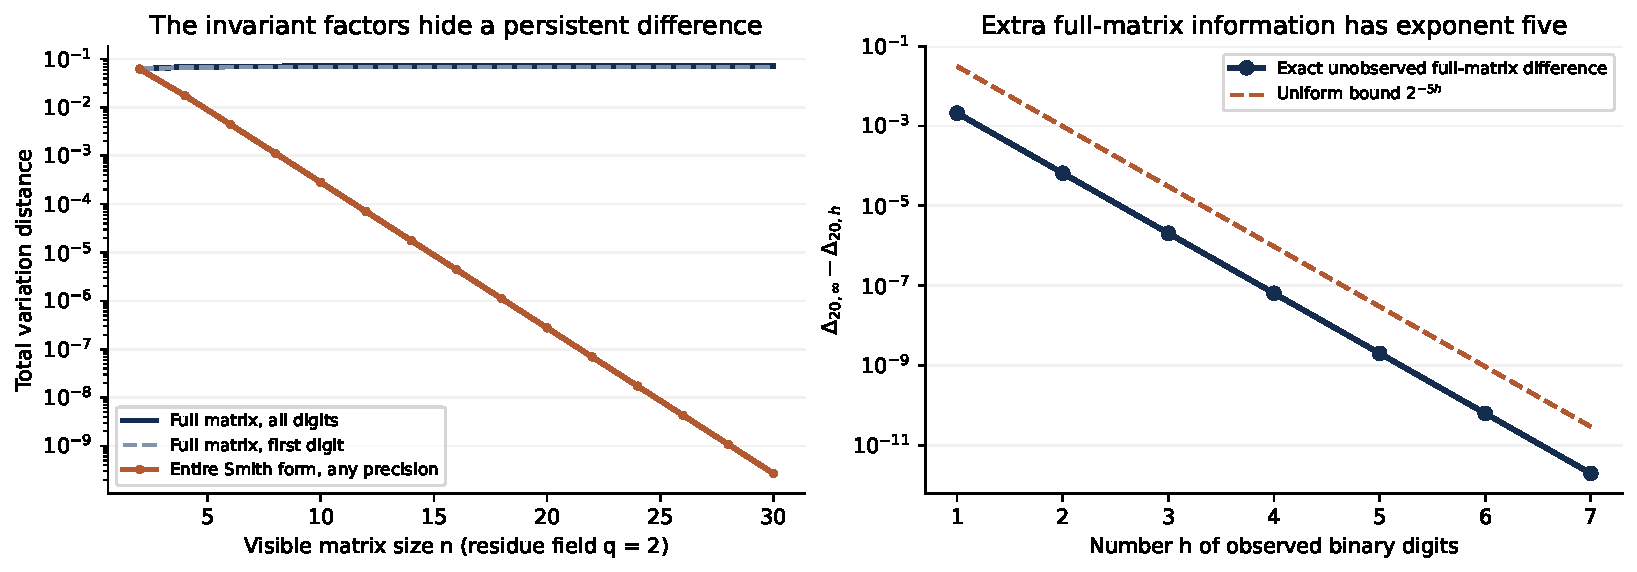
\includegraphics[width=.96\linewidth]{figures/precision_separation.pdf}
 \caption{Separation between the full-matrix and Smith-form laws,
 computed from the exact formulas. The full-matrix precision error
 obeys the sharp fifth-power law, whereas the Smith testing distance
 is independent of precision.}
 \label{fig:local-separation}
\end{figure}

The theorem therefore identifies both the information retained and the
information discarded by Smith normal form: the invariant factors
retain the entire module structure, while the alternating form on the
successive kernel modules carries an additional persistent constraint.

